% AI workflow slide, standalone copy of slide 27 of talk/slides.tex.
% Written by Claude Opus 5.5 (Claude Code), 2026-11-14. Preamble copied from talk/slides.tex.
\documentclass[aspectratio=169,11pt]{beamer}
\usetheme{default}
\usecolortheme{seahorse}
\setbeamertemplate{navigation symbols}{}
\setbeamertemplate{footline}[frame number]
\setbeamercolor{frametitle}{fg=blue!50!black}
\setbeamercolor{title}{fg=blue!50!black}
\usepackage{amsmath,amssymb}
\usepackage{tikz}
\usepackage{pifont}
\usetikzlibrary{arrows.meta,positioning}
% colours shared with talk/figures/make_figures.py (symmetric = blue circle, asymmetric = orange square)
\definecolor{symblue}{HTML}{2A78D6}
\definecolor{asymorange}{HTML}{EB6834}
\definecolor{atomgreen}{HTML}{1BAF7A}

% ---- status switches: change these two lines after human sign-off ----
\newcommand{\claimstatus}{candidate proof, under verification}
\newcommand{\ourresult}{Claim}
% --------------------------------------------------------------------
\newcommand{\status}{\par\vfill{\tiny\color{gray}\claimstatus\par}}
\newcommand{\vp}{v_p}
\newcommand{\sd}{s_p}
\newcommand{\Z}{\mathbb{Z}}
\newcommand{\Cq}{C_n^{(q)}}
\DeclareMathOperator{\Fix}{Fix}

\tikzset{
  intnode/.style={circle,draw,fill=black,inner sep=1.4pt},
  symnode/.style={circle,draw=white,fill=symblue,inner sep=2.2pt},
  asymnode/.style={rectangle,draw=white,fill=asymorange,inner sep=2.7pt},
  leafdot/.style={circle,draw,fill=white,inner sep=1.2pt},
  atom/.style={regular polygon,regular polygon sides=3,draw=atomgreen,fill=atomgreen!18,
               inner sep=1pt,minimum size=9mm,font=\small},
  treeedge/.style={draw,thick}
}
\usetikzlibrary{shapes.geometric}
\begin{document}

% 16b ----------------------------------------------------------------
% Infrastructure slide. Written by Claude Opus 5.5 (Claude Code), 2026-11-14.
\begin{frame}{How the AI team worked: every claim runs the gauntlet}
  \vspace{-4pt}
  \centering
  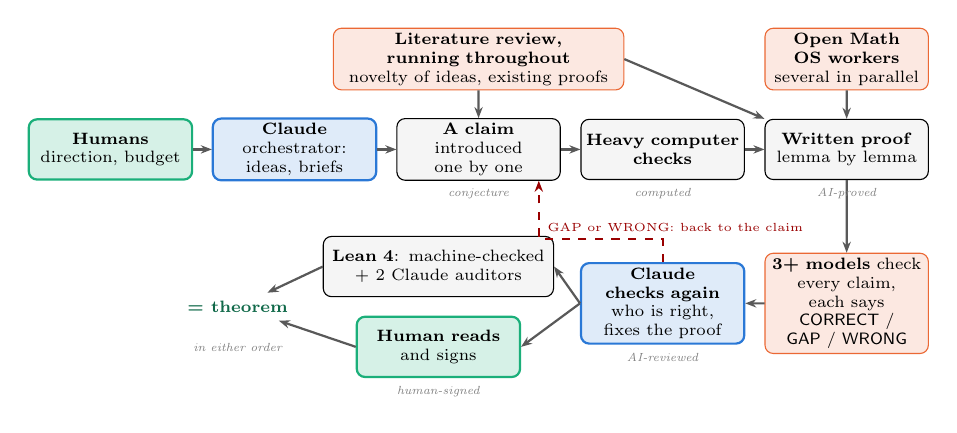
\begin{tikzpicture}[scale=0.85,transform shape,
      st/.style={draw,rounded corners=3pt,align=center,inner sep=2pt,
                 text width=23mm,minimum height=9mm,font=\scriptsize,fill=gray!8},
      ag/.style={st,fill=asymorange!15,draw=asymorange},
      cl/.style={st,fill=symblue!15,draw=symblue,thick},
      hu/.style={st,fill=atomgreen!18,draw=atomgreen,thick},
      gr/.style={font=\tiny\itshape,text=gray},
      fl/.style={-{Stealth[length=4pt]},thick,gray!70!black},
      fb/.style={-{Stealth[length=4pt]},thick,dashed,red!60!black}]
    % top row, left to right
    \node[hu] (H)  at (0,0)     {\textbf{Humans}\\ direction, budget};
    \node[cl] (O)  at (2.75,0)  {\textbf{Claude}\\ orchestrator:\\ ideas, briefs};
    \node[st] (C)  at (5.5,0)   {\textbf{A claim}\\ introduced one by one};
    \node[st] (X)  at (8.25,0)  {\textbf{Heavy computer}\\ \textbf{checks}};
    \node[st] (P)  at (11,0)    {\textbf{Written proof}\\ lemma by lemma};
    % helpers above
    \node[ag,text width=42mm] (L)  at (5.5,1.35)
      {\textbf{Literature review, running throughout}\\ novelty of ideas, existing proofs};
    \node[ag] (W)  at (11,1.35)   {\textbf{Open Math OS workers}\\ several in parallel};
    % bottom row, right to left
    \node[ag] (R)  at (11,-2.3)   {\textbf{3+ models} check\\ every claim, each says\\ \textsf{CORRECT / GAP / WRONG}};
    \node[cl] (A)  at (8.25,-2.3) {\textbf{Claude checks again}\\ who is right,\\ fixes the proof};
    \node[st,text width=33mm] (K)  at (4.9,-1.75) {\textbf{Lean 4}: machine-checked\\ + 2 Claude auditors};
    \node[hu] (S)  at (4.9,-2.95) {\textbf{Human reads}\\ and signs};
    \node[font=\scriptsize\bfseries,text=atomgreen!60!black] (T) at (1.9,-2.35) {= theorem};
    % flow
    \draw[fl] (H) -- (O); \draw[fl] (O) -- (C); \draw[fl] (C) -- (X); \draw[fl] (X) -- (P);
    \draw[fl] (L) -- (C); \draw[fl] (L.east) -- (P.north west);
    \draw[fl] (W) -- (P);
    \draw[fl] (P) -- (R); \draw[fl] (R) -- (A);
    \draw[fl] (A.west) -- (K.east); \draw[fl] (A.west) -- (S.east);
    \draw[fl] (K.west) -- (T); \draw[fl] (S.west) -- (T);
    \draw[fb] (A.north) -- ++(0,0.35) -| node[pos=0.6,right,font=\tiny,text=red!60!black,align=left]{GAP or WRONG: back to the claim} ([xshift=9mm]C.south);
    % grades of the claim ledger
    \node[gr,below=0pt of C] {conjecture};
    \node[gr,below=0pt of X] {computed};
    \node[gr,below=0pt of P] {AI-proved};
    \node[gr,below=0pt of A] {AI-reviewed};
    \node[gr,below=0pt of S] {human-signed};
    \node[gr,below=6pt of T] {in either order};
  \end{tikzpicture}

  \vspace{1pt}
  {\scriptsize
  \textcolor{atomgreen}{\rule{7pt}{7pt}} humans \quad
  \textcolor{symblue}{\rule{7pt}{7pt}} Claude (orchestrator) \quad
  \textcolor{asymorange}{\rule{7pt}{7pt}} other AI agents and models \quad
  \textcolor{gray!45}{\rule{7pt}{7pt}} claims, checks and proofs \par}

  \vspace{3pt}
  \raggedright\scriptsize
  \begin{itemize}\setlength{\itemsep}{0pt}
    \item Open Math OS agents work for Claude, several running in parallel;
      everything the sub-agents output is checked again by Claude.
    \item Everything is recorded. That gives transparency, and the journal and state file
      let an agent that stopped running for whatever reason pick up with full context.
    \item Every worker run is logged automatically.
    \item Every file and statement is marked: verified by a human or not, and if an AI made it,
      which specific AI.
  \end{itemize}
\end{frame}

% 16c ----------------------------------------------------------------
% Results slide. Written by Claude Opus 5.5 (Claude Code), 2026-11-15.
% Statuses as in CLAIMS.md and report/report.tex, Section "Limitations".
\begin{frame}{What we achieved: four proofs of Problem 137}
  \centering
  \renewcommand{\arraystretch}{1.6}
  \begin{tabular}{lcc}
    & \textbf{Lean verified} & \textbf{Human checked} \\ \hline
    Lattice paths             & \textcolor{atomgreen}{\ding{51}} & read, no gaps found \\
    Algebraic (Frobenius)     & \textcolor{atomgreen}{\ding{51}} & not verified \\
    Accounting                & \textcolor{atomgreen}{\ding{51}} & read, no gaps found \\
    Main: symmetries of trees & \textcolor{atomgreen}{\ding{51}} & rigorously verified \\
  \end{tabular}

  \vspace{14pt}
  {\small Lean verified: builds on Lean v4.35.0 / Mathlib, no \texttt{sorry}, standard axioms only.\par}
\end{frame}

\end{document}
